%%%%%%%%%%%%%%%%%%%%%%%%%%%%%%%%%%%%%
%% Supporting Information
%% (Optional)
%%%%%%%%%%%%%%%%%%%%%%%%%%%%%%%%%%%%%
% OVERVIEW
%
% Please note that all supporting information will be peer reviewed with your manuscript.
% In general, the purpose of the supporting information is to enable
% authors to provide and archive auxiliary information such as data
% tables, method information, figures, video, or computer software,
% in digital formats so that other scientists can use it.

% The key criteria are that the data:
% 1. supplement the main scientific conclusions of the paper but are not essential to the conclusions (with the exception of
%    including data so the experiment can be reproducible);
% 2. are likely to be usable or used by other scientists working in the field;
% 3. are described with sufficient precision that other scientists can understand them, and
% 4. are not exe files.
%

% All Supporting text and figures should be included in this document.

% Data sets, large tables, movie files,
% and audio files should be uploaded separately, following AGU naming
% conventions. Include their captions in this document and list the
% file name with the caption. You will be prompted to upload these
% files on the Upload Files tab during the submission process, using
% file type “Supporting Information (SI)”

%\documentclass{agujournal2018}

% Please type in the journal name: \journalname{<Journal Name>}
% ie,
%\journalname{Journal of Geophysical Research: Solid Earth}

%% Choose from this list of Journals:
%
% Journal of Geophysical Research
% JGR-Biogeosciences
% JGR-Earth Surface
% JGR-Planets
% JGR-Solid Earth
% JGR-Space Physics
% Global Biochemical Cycles
% Geophysical Research Letters
% Paleoceanography
% Radio Science
% Reviews of Geophysics
% Tectonics
% Space Weather
% Water Resource Research
% Geochemistry, Geophysics, Geosystems
% Journal of Advances in Modeling Earth Systems (JAMES)
% Earth's Future
% Earth and Space Science

\documentclass[main.tex]{subfiles}

\begin{document}

%% This command needs article title as argument to \supportinginfo{}:
%\supportinginfo{Enhanced Dehydration Weakening of Antigorite Driven by Slow Shear Heating: Insights from High-Pressure Experiments with a Modified Apparatus Stiffness}

%\authors{Eric Burdette and Greg Hirth}

%\affiliation{1}{Department of Earth, Environmental and Planetary Sciences, Brown University, Providence, RI, USA}

%% Corresponding Author
%(include name and email addresses of the corresponding author.  More
%than one corresponding author is allowed in this Word file and for
%publication; but only one corresponding author is allowed in our
%editorial system.)  

%\correspondingauthor{Eric Burdette}{eric\_burdette@brown.edu}


%% ------------------------------------------------------------------------ %%
%
%  TEXT
%
%% ------------------------------------------------------------------------ %%

\section{Supporting Information}

% \section*{Contents}
% %%%Remove or add items as needed%%%
% \begin{enumerate}
% \item Text S1 to S6
% \item Figures S1 to S5
% \end{enumerate}

% \section*{Introduction} 
% Included below are supporting information including descriptions of temperature rise calculation methods, stiffness estimation and calibration methods, experimental assembly notes, a section exploring connections of current data to previous work in the quantities they used, and a supporting figure of sample structure evolution.
%Delete all unused file types below. 
%Copy/paste for multiples of each file type as needed.

\subsection{Thermal Model}

The temperature rise predicted for the center of deforming gouge layer was calculated using an analytical expression that considers distributed shear work and thermal conduction.
\begin{equation}
    T\left(y,t\right)=T_0+\int_{0}^{t}\frac{\tau\left(t^\prime\right)V\left(t^\prime\right)}{\rho c\sqrt{2\pi}}\frac{1}{\sqrt{W^2+2\alpha_{th}\left(t-t^\prime\right)}}exp\left(-\frac{y^2}{2W^2+4\alpha_{th}\left(t-t^\prime\right)}\right)dt^\prime\
    \label{eq:S1}
\end{equation}

The details are described in Proctor et. al (2014). The shear stress ($\tau$ ) was calculated as half of the differential stress. We are interested in peak temperature so we report values for y = 0. Velocity (V) was calculated for the shear surface of the 45° saw-cut piston from the axial displacement rate of the sample ($V_{sample}$). In the calculations we use a deforming gouge layer half-width (W) of 100 $\mu$m, a thermal diffusivity ($\alpha_{th}$) of $10^{-6}$ m2/s, and a volumetric heat capacity ($\rho_c$) of 2.7x$10^6$ Pa/°C (Proctor et. al 2014).  The half width only becomes important when $W^2$ is much larger than $\alpha_{th}\left(t-t^\prime\right)$, i.e., at very short times, or very large W. With large W, the heat is already widely distributed so thermal diffusivity is less important, and at short times heat cannot migrate quickly so temperature rise is strongly dependent on amount of material the heat is generated in.
For reference, shear and normal ($\sigma_n$) stresses in triaxial geometry can be computed with relationships for Mohr’s circle from Jaeger et. al. (2007), where axial force is $\sigma_1$ and confining pressure is $\sigma_3$.
\begin{equation} \label{eq:S2}
    \tau=\frac{\sigma_1-\sigma_3}{2}sin(2\theta)
\end{equation}
\begin{equation} \label{eq:S3}
    \sigma_n=\frac{\sigma_1+\sigma_3}{2}-\frac{\sigma_1-\sigma_3}{2}cos(2\theta)\ 
\end{equation}
Temperatures were calculated with area corrected shear stress. The area correction is calculated with a relation for the overlap of two ellipses presented in the RIG 1.3 by Matej Pec. The contact area change can be calculated as a function of piston shear. 
\begin{equation} \label{eq:S4}
    contact\ length=\ c\ =\frac{shear\ displacement}{starting\ shear\ length}\ =\frac{\Delta x_{axial}}{Diameter}tan(\theta)
\end{equation}
where $\theta$ is angle between the saw-cut and piston axis.  The area is then calculated as:
\begin{equation} \label{eq:S5}
    \frac{A}{A_0}=1-1.2082\ \times c\ -\ 0.19134\ \times c^2\ +\ 0.39461\times c^3\ 
\end{equation}
\begin{equation} \label{eq:S6}
    \tau_{corrected}(t)=\tau_{measured}(t)\frac{A_0}{A}\
\end{equation}

Sample temperatures do not significantly lag the temperature ramp set point. This can be estimated based on solutions for diffusion in an infinite cylinder. For this calculation we use an alumina thermal conductivity of $10^{-5} m^2$/s because the shearing pistons make up most of jacketed cylinder’s volume.  The thermocouple is 3 mm away from the center of the sample. The center of the sample will reach 98\% of an instantaneous temperature change in less than 1s (based on a normalized time of $0.8=\alpha_{th\ Al2O3}t/{0.003}^2$; Figure 12, Carslaw and Jaeger, 1959). For example, if we could instantaneously increase surface temperature by 300°C, the center of the sample would reach 294 °C in 0.8 seconds. Thus, for a temperature ramp rate of 0.5°C /s the temperature will not lag behind the setpoint by more than 1°C over the duration of the temperature ramp (which is on order of the error in our temperature measurement).

\subsection{Compliance with the general shear assembly}
    The area offset on the shear pistons used in the general shear geometry affects both stress state (as noted above) and the effective shear stiffness (i.e., the change in gouge stress with shear displacement). As the sample slips during weakening, the spring unloads, but area between the pistons is also getting smaller. This effectively decreases sample stiffness. While the overlapping area of the pistons is getting smaller between pistons, the force/displacement relationship of the spring stays the same, leading to an increase in the instantaneous stiffness of the column (this is a competing effect). As slip continues, the change in overlapping area with displacement decreases ($dA_{overlap}/ds$ decreases). In our experiments, rapid slip and the onset of reaction starts after relatively low displacement, so this effect does not affect our conclusions.
    
\subsection{D-DIA Stiffness}
    The stiffness of the D-DIA apparatus was calculated from elastic stiffness of steel deformation anvils and hydraulic fluid compressibility. 
    First, the frame is assumed to be infinitely stiff. The hydraulic ram radius is 44.5 mm, and total stroke is 20 $cm^3$ (Wang et al., 2003). Bulk modulus of the oil is assumed to be 1.5 GPa. Compressing this volume of oil to 50 MPa with the ram would lead to ram force of 311 kN and displacement of 0.333 mm. On a 1.2mm diameter sample used in Hilairet et al (2007) this is 275 GPa which results in a stiffness of 825 GPa/mm. The same calculation from specification given in Ferrand et al 2017, with a 2.1 mm diameter sample gives a stiffness of 270 GPa/mm. 
    The internal steel ram stiffness can be estimated approximately as a cone with diameters 10 mm and 90 mm. Integrating displacement along the cone length with elastic modulus of 200 GPa gives elastic displacement of 0.99 mm at 311 kN for a stiffness of 278 GPa/mm and 91 GPa/mm respectively (1.2, 2.1 mm diameter).  
    The composite stiffness (combining the hydraulic stiffness and the steel ram stiffness) for Hilairet et al. 2007 condition is 208 GPa/mm; this is the value quoted in the text of our paper. Substantial uncertainty exists due to friction in the sample assembly so effective stiffness on the sample could be much larger.
    
\begin{figure}
    \centering
    \includegraphics[width=\textwidth]{Figures/S1 - Copy.pdf}
    \caption[Mechanical model of apparatus compliance]{Schematic drawing of the components of the loading frame and column drawn in a realistic style and a typical 1D mechanics style alongside the typical schematic of a 1D rate-state friction slider block model.  Change in displacement of all the loading elements (zigzag lines) for a change in sample load need to be accounted for to form the typical $K_{Apparatus}$ used in rate-state models.}
    \label{fig:S1}
\end{figure}    
\begin{figure}
    \centering
    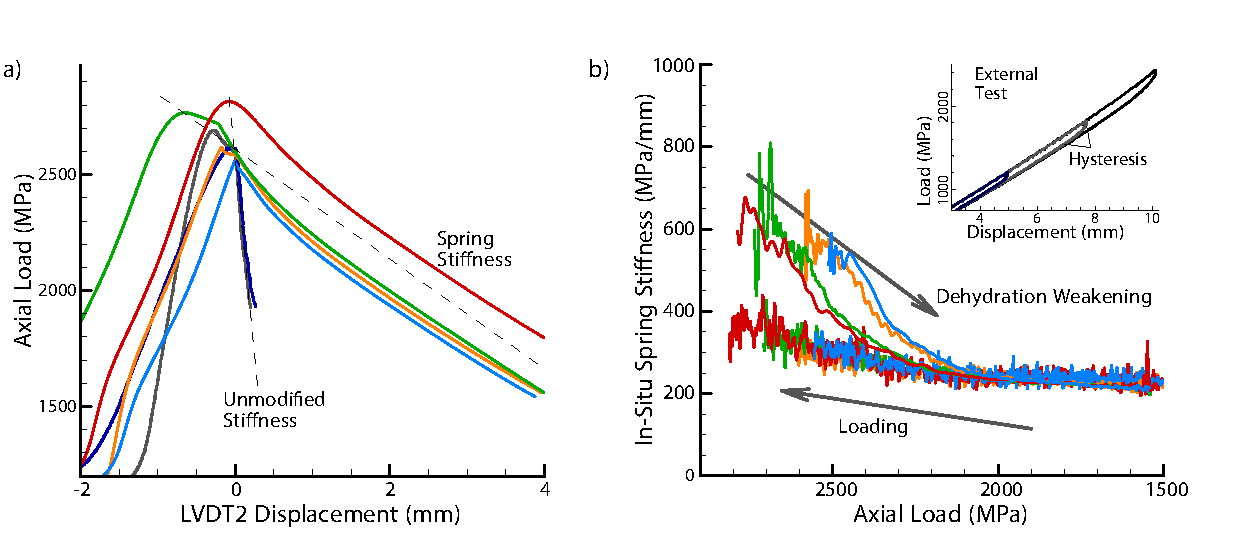
\includegraphics[width=\textwidth]{Figures/S2 - Copy.pdf}
    \caption[Figures summarizing recorded load, displacement, and stiffness during experiments]{Figures summarizing recorded load, displacement, and their derivative relationship (stiffness). (a) Load plotted against displacement for dehydration runs, with displacement referenced to the recorded value at initiation of the temperature ramp. Dashed reference lines are plotted for the static stiffness of the standard and modified apparatus. (b) Absolute value of instantaneous absolute spring stiffness measured for the load-displacement curves in (a) (both loading and weakening). Inset shows separate results of calibration experiments on only the spring elements using a hydraulic press; the frictional hysteresis matches the observed unloading behavior during the dehydration experiments.}
    \label{fig:S2}
\end{figure}

\subsection{Measurement of apparatus, column, and spring stiffness}
    Disambiguation of measured stiffnesses is important for interpretation of data and comparison to other studies. It is simple to consider the stiffness of the whole rig as a loop of springs, with the frame expanding/returning and the loading column compressing/expanding as load changes in the loop due to advancing/retracting the ball screw or slipping the sample, respectively. Our LVDTs are positioned close to, but not directly on the sample (see Figure \ref{fig:F2} and Figure \ref{fig:S1}). This divides the stiffness of the whole rig, $K_{apparatus}$, into two halves: $K_{upper\ column}$ and $K_{lower\ column}$.

\begin{figure}
    \includegraphics[width=\textwidth]{Figures/SuppTableSnip.png}
    \caption{Apparatus compliance measurements.}
    \label{fig:tableS1}
\end{figure}

    We can introduce displacement in either section of the loop to measure elastic stiffness of the other half (e.g. ball screw to measure to lower pistons and anvil, or hydraulic jack in place of sample to measure springs, load cell, ball screw, and frame). In Figure \ref{fig:S1}, the ball screw displacement is noted as $x_0$ and the sample or hydraulic jack displacement is noted as $x_{sample}$. The resulting combination of the stiffness of the two halves is the value that the sample responds to (“feels”) during slip (or propagation of instabilities) so the combination of the whole loop (Kapparatus) should be used for assessment of stability. 
    Mathematically the stiffnesses can be expressed as:
    \begin{equation} \label{eq:S7}
        K_{Measured}=\frac{dF}{dx_{LVDT2}}
    \end{equation}
    \begin{equation} \label{eq:S8}
        \frac{1}{K_{Lower\ Column}}=\frac{1}{K_{Pistons}}+\frac{1}{K_{Base\ Anvils}}
    \end{equation}
    \begin{equation} \label{eq:S9}
        \frac{1}{K_{Upper\ Column}}=\frac{1}{K_{Frame}}+\frac{1}{K_{Ball Screw}}+\frac{1}{K_{Load\ Cell}}+\frac{1}{K_{Disk\ Springs}}
    \end{equation}
    \begin{equation} \label{eq:S10}
        \frac{1}{K_{Apparatus}}=\frac{1}{K_{Lower\ Column}}+\frac{1}{K_{Upper\ Column}}
    \end{equation}
    
    For simplicity, our rig schematic omits the hydraulic ram, which applies 1 GPa pressure to our 1 inch diameter pressure vessel. This omission is negligible if pressure remains constant or varies by only a small amount. We satisfy this condition by ramping temperature at 0.5°C/s, which produces only a small change in pressure. In contrast, if pressure changes by a large amount (~100 MPa -> ~100 µm expansion) over a short period (for example, in 1 minute for a temperature ramp rate of 5°C/s at $V_0\-2$µm/s), the hydraulic ram force adds to frame expansion and pushes the top platen up. The upward motion is applied in the opposite direction of ball screw displacement ($V_0$) which changes effective $V_0$ substantially and can even unload samples.
    
    Okazaki et al. (2015) choose to report their stiffness as a shear quantity so it needs to be converted to an axial quantity for comparison. Their reported effective force-displacement from stress drops in the supplement is 80kN/mm on 20 mm diameter pistons which have an area of 314 $mm^2$ which results in an axial stiffness of 254 MPa/mm. The reported shear stiffness in the main text can be converted to axial stiffness by using constant pressure derivatives of equation \ref{eq:S2} and conversion of shear to axial displacement ($cos(\theta)$). The conversion of their stated 58 MPa/mm shear stiffness to axial stiffness results in axial apparatus stiffness of 155 MPa/mm. They do not draw a stiffness diagram or note at which two points on their machine the displacement is measured, so it is unclear whether 155 MPa/mm is the entire machine ($K_{Apparatus}$) or another value. Nonetheless we use 155 MPa/mm for a relative comparison.


\subsection{Nonlinear Elastic Spring Behavior}
    During dehydration experiments with the modified stiffness, the initial weakening occurs with a steeper slope in the recorded load-displacement curves (Figure \ref{fig:S2}a). We isolated the load displacement relationship for the Belleville disk spring stack during these experiments by taking the difference in displacement between LVDT1 and LVDT2. We found that the spring stack was the source of the nonlinear elasticity, with an initially large drop in force/load after either weakening or unloading started. This is a known effect in Belleville disk spring stacks due to frictional contact between the disks. We confirmed this hysteresis by compressing the stack (instrumented with a direct LVDT) in an external press (Figure \ref{fig:S2}b).
    
\subsection{Notes on Relationships Among Unloading Slope, $V_0$, and Unloading Rate}
    To investigate the influence of dehydration reactions on weakening slope, we analyze stress relaxation of a frictional slider-block in the context of previous work that focused on relationships among measured $\frac{{dF}}{{d}{x}_{{LVDT}}}$ , $V_0$, reaction rate, and $K_{upper\ column}$,  (referred to for this section as just K) stiffness (e.g., Okazaki et al. 2016, Chernak et al. 2011; Figure \ref{fig:S4}). For quasi-static (no effect of inertia) conditions, the change in force during weakening of a slider block is directly proportional to the apparatus stiffness (K):
    \begin{equation} \label{eq:S11}
        \frac{{dF}}{{dt}}={K}_{{upper}\ {column}}\left({V}_{0}-{V}_{{LVDT}{2}}\right)
    \end{equation}
    which can be rearranged to define a relationship for the sample displacement rate:
    ${V}_{{LVDT}}={V}_{0}-\frac{{dF}}{{dt}}\frac{{1}}{{K}}$ .  The unloading slope is determined from the observed change in force and displacement, which from substitution for $V_{sample}$ can be written as:
    \begin{equation} \label{eq:S12}
     \frac{dF}{dx}=\frac{\frac{{dF}}{{dt}}}{\frac{{dx}}{{dt}}}=\frac{\frac{{dF}}{{dt}}}{{V}_{{LVDT}}} =\frac{\frac{{dF}}{{dt}}}{{V}_{0}-\frac{{dF}}{{dt}}\frac{{1}}{{K}}}={K}\frac{\frac{{dF}}{{dt}}}{{V}_{0}{K}-\frac{{dF}}{{dt}}}
    \end{equation}

\begin{figure}
    \centering
    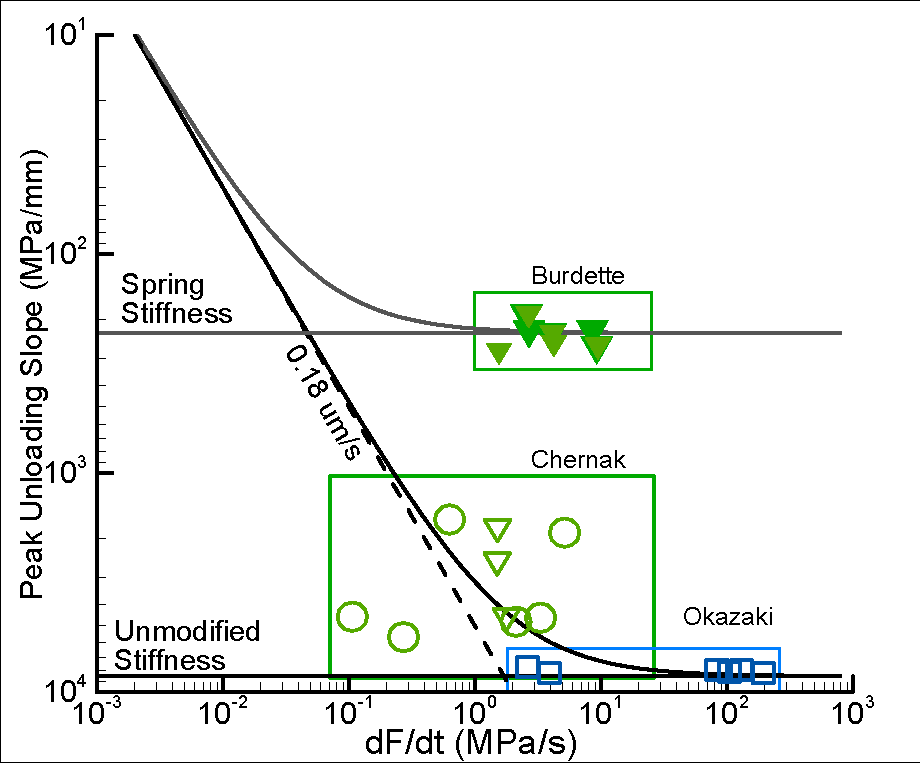
\includegraphics[width=\textwidth]{Figures/S4 - Copy.pdf}
    \caption[Plot of unloading slope vs. weakening rate]{Mechanical description of apparatus unloading during sample weakening following equation \ref{eq:SH3}. Peak weakening slope calculated from compliance is plotted against unloading rate to illustrate the transition between regimes and where previous experimental work trends relative to this work. Open symbols are unmodified apparatus runs. Circles are data from Chernak and Hirth (2011), squares are lawsonite runs from Okazaki and Hirth (2016), inverted triangles are this work. Note reference $K_{upper compliance}$ is \~3x larger than quoted in this study due to placement of LVDT1 used in these older studies.}
    \label{fig:S4}
\end{figure}

    Equation (\ref{eq:S12}) has three regimes: (i) with ${V}_{0}{K}\gg\frac{{dF}}{{dt}}$, the unloading slope approaches $\frac{\frac{{dF}}{{dt}}}{{V}_{0}}$ (with the limiting case of dF/dx = 0 for steady state sliding); (ii) an intermediate regime which follows equation (\ref{eq:S12}); and (iii) with ${V}_{0}{K}\ll\frac{{dF}}{{dt}}$, the unloading slope approaches K (a limiting case that includes scenarios related to stick-slip (i.e., large dF/dt) or stress relaxation with a fixed loadpoint (i.e. Vo ≈ 0). As illustrated in Figure \ref{fig:S4}, the experiments showing stable slip during dehydration of antigorite (Chernak et al. 2011, Okazaki et al. 2016) fall in either regime (i) or regime (ii); the unstable slip associated with dehydration of lawsonite (Okazaki et al. 2016) falls in regime (iii) for a limiting case in which stick-slip is observed; and the unloading slope observed in our new experiments with the modified stiffness falls in regime (iii) for the limiting case of an effectively fixed load point displacement. For comparison to earlier work, the data from these studies are summarized in Figure \ref{fig:S4} on a plot of dF/dx versus temperature ramp rate over strain rate.

\begin{figure}
    \includegraphics[width=\textwidth]{Figures/S5 - Copy.pdf}
    \caption[Summary SEM mosaics of interrupted and dehydrated samples]{Modified compliance dehydration specimens showing deformation patterns and reacted zones.  Upper two images show samples that were quenched after ramping from 400-600°C, while the bottom micrograph was quenched after the sample was fully relaxed after ramping to 700°C. The uppermost image was hydrostatically loaded and preserves initial grain shapes with no signs of reaction evident. The middle image (W2319) shows formation of localized fracture bands along the R1 shear direction which accommodate most of the sample slip (see Figure \ref{fig:F6}). The lower image shows a high displacement deformed sample (W2333), with darker areas near the center of the specimen showing high reaction extent.}
    \label{fig:S5}
\end{figure}





\end{document}